\subsubsection{Use Case}
Here follows the use case diagram: \\

\begin{figure}[H]
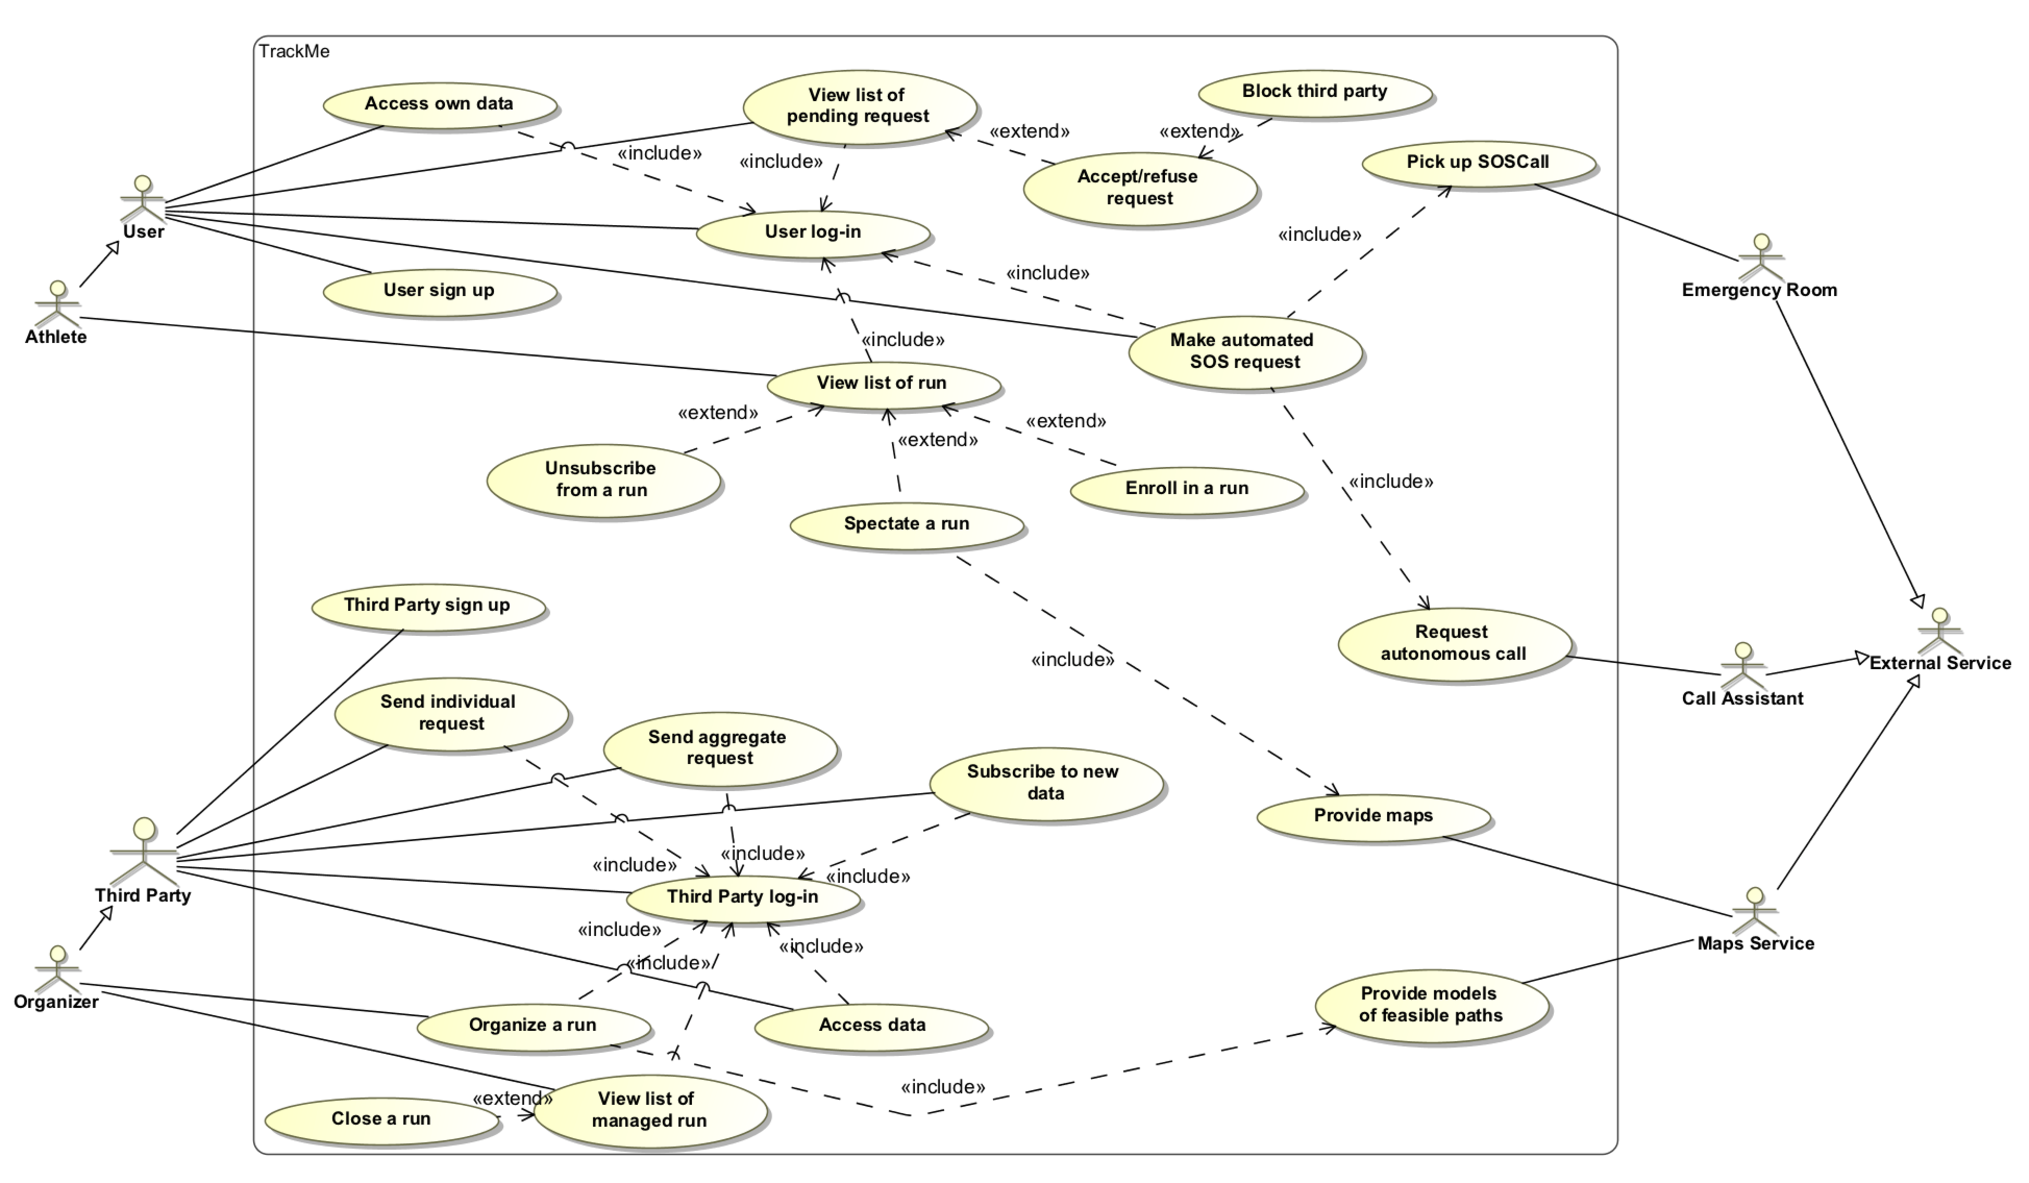
\includegraphics[width=\linewidth]{Images/usecase}
\caption{Use case diagram}
\label{fig:usecasediagram}
\end{figure}

\par 
Beneath, the use case is analyzed:	\\

\begin{table}[H]
\begin{tabularx}{\textwidth}{|l|X|}
\hline
 Name & Send aggregated request \\ \hline
 Actor & Third party customer  \\ \hline
 Entry conditions & Third party customer needs some aggregated data on anonymized users and the third party has performed log-in \\ \hline
 Event flow & 
 \begin{enumerate}
 	\item Third party customer compiles a form specifying the aggregated data that he wants to access
 	\item Third party customer sends the request
 	\item The system analyses the request and provides to the user the access to the data 
 \end{enumerate}   \\ \hline
 Exit conditions & The third party user can access the requested data \\ \hline
 Exceptions & If the request involves less or equal than 1000 distinct user, the access is not provided to the third party that gets a notification \\ \hline
\end{tabularx}
\end{table}

\begin{table}[H]
\begin{tabularx}{\textwidth}{|l|X|}
\hline
 Name & Subscribe to new data \\ \hline
 Actor & Third party customer  \\ \hline
 Entry conditions & Third party customer needs some future aggregated data on anonymized users and the third party has performed log-in \\ \hline
 Event flow & 
 \begin{enumerate}
 	\item Third party customer compiles a form specifying the future aggregated data that he wants to access, when they will be available
 	\item Third party customer sends the request
 	\item The system waits for the moment in which all the future data requested will be generated 
 	\item The system analyses the request and provides to the user the access to the data 
 \end{enumerate}   \\ \hline
 Exit conditions & The third party user can access the requested data \\ \hline
 Exceptions & If the request involves less or equal than 1000 distinct user, the access is not provided to the third party that gets a notification \\ \hline
\end{tabularx}
\end{table}

\begin{table}[H]
\begin{tabularx}{\textwidth}{|l|X|}
\hline
 Name & Make autonomous SOS call \\ \hline
 Actor & User, emergency room operator \\ \hline
 Entry conditions & User health parameters detected below the threshold for the first time in an hour \\ \hline
 Event flow & 
 \begin{enumerate}
 	\item The mobile application calls autonomously the emergency number 
 	\item The emergency room operator picks the call up 
 	\item The mobile applications communicates the health parameters and the user location to the emergency room operator, thus requesting for assistance 
 	\item The emergency room operator accepts the request
 	\item The emergency room operator sends an ambulance to the user location
 \end{enumerate}   \\ \hline
 Exit conditions & An ambulance is sent to the user location \\ \hline
 Exceptions & If the emergency room operator refuses the request, a warning is sent to the user \\ \hline
\end{tabularx}
\end{table}

\begin{table}[H]
\begin{tabularx}{\textwidth}{|l|X|}
\hline
 Name & Organize run \\ \hline
 Actor & Third party customer \\ \hline
 Entry conditions & The third party customer has performed login and needs to organize a race\\ \hline
 Event flow & 
 \begin{enumerate}
 	\item The third party customer set up a run: he provides the name, the path, the date, the starting time, a closure date for the subscriptions and the minimum number of participants
  	\item The third party customer sends all the mentioned above information to the system
 	\item The system adds the run to the list of the available races
 \end{enumerate}   \\ \hline
 Exit conditions & The race has been successfully added to the list of the available run \\ \hline
 Exceptions & 
 \begin{enumerate}
 	\item The name is already used by another run
 	\item Another run is already been specified for the same date and at least a portion of the path is overlapping 
 \end{enumerate}  
 All the exceptions are handled in the same way: the race is not added to the list and the third party user gets notified of the unsuccessful operation 
 \\ \hline
\end{tabularx}
\end{table}


\begin{table}[H]
\begin{tabularx}{\textwidth}{|l|X|}
\hline
 Name & Enroll in a run \\ \hline
 Actor & Athlete \\ \hline
 Entry conditions & The user wants to join to a run that has previously been added to the list of the available race \\ \hline
 Event flow & 
 \begin{enumerate}
 	\item The athlete accesses the list of available run
  	\item The athlete selects the race in which he wants to enroll
 	\item The athlete sends the request for joining the run to the system 
 	\item The system receives the requests and enroll the athlete in the race that he has specified 
 \end{enumerate}   \\ \hline
 Exit conditions & The athlete has been successfully enrolled to the race \\ \hline
 Exceptions &  
 \begin{enumerate}
 	\item The athlete is already enrolled to the race that he specifies in the request
 	\item The athlete is already been enrolled to a race in the same date of the run specified in the request 
 \end{enumerate}
 All the exceptions are handled in the same way: the athlete is notified that the enrollment was unsuccessful, by providing a brief motivation. Of course, the subscription process is aborted  
 \\ \hline
\end{tabularx}
\end{table}


\begin{table}[H]
\begin{tabularx}{\textwidth}{|l|X|}
\hline
 Name & Block requests from a company \\ \hline
 Actor & User \\ \hline
 Entry conditions & The user wants to block the request from a specific company and the company has sent to the user a request \\ \hline
 Event flow & 
 \begin{enumerate}
 	\item The user accesses the list of available requests
  	\item The user refuses a pending request 
 	\item The user blocks the company that has sent the request
 	\item The system receives the user's decision and permanently blocks the company that has sent the request
 \end{enumerate}   \\ \hline
 Exit conditions & The company has been successfully blocked \\ \hline
 Exceptions &  No exceptions
 \\ \hline
\end{tabularx}
\end{table}


\begin{table}[H]
\begin{tabularx}{\textwidth}{|l|X|}
\hline
 Name & Accept request\\ \hline
 Actor & User \\ \hline
 Entry conditions & The user wants to accept a request that a company has sent to the user and the request is in the pending request list \\ \hline
 Event flow & 
 \begin{enumerate}
 	\item The user accesses the list of available requests
  	\item The user selects the request which he wants to accept
 	\item The user accepts the request from a specific company
 	\item The system receives the acceptance and notifies both the third party and the user of the successful of the operation
 \end{enumerate}   \\ \hline
 Exit conditions & The data specified in the request is now accessible to the third party that has sent the request that has been accepted\\ \hline
 Exceptions & No exceptions
 \\ \hline
\end{tabularx}
\end{table}


\begin{table}[H]
\begin{tabularx}{\textwidth}{|l|X|}
\hline
 Name & Sign up \\ \hline
 Actor & User \\ \hline
 Entry conditions & The user wants to utilize the application, but he has not registered yet \\ \hline
 Event flow & 
 \begin{enumerate}
  	\item The user completes the registration's form and provides his information
 	\item The user sends the information to the system
 	\item The system checks that an account associated with the specified credentials does not exist
 	\item The system checks that an account associated with the specified social security number does not exist
 	\item The system checks that an account associated with the specified username does not exist
 	\item The system registers the user into the application
 \end{enumerate}   \\ \hline
 Exit conditions & The user is successfully been registered \\ \hline
 Exceptions & The user provides non-valid data: credential or username or social security number has already been used in another successful registration process. In this case, the user is notified that the subscription is unsuccessful, by providing a brief motivation. 
 \\ \hline
\end{tabularx}
\end{table}


\begin{table}[H]
\begin{tabularx}{\textwidth}{|l|X|}
\hline
 Name & Login \\ \hline
 Actor & User \\ \hline
 Entry conditions & The user wants to use the application and he is already registered \\ \hline
 Event flow & 
 \begin{enumerate}
 	\item The user sends his username and password credentials through the application
  	\item The system checks the information provided by the user
 	\item The system provides access to the user to the TrackMe services
 \end{enumerate}   \\ \hline
 Exit conditions & The user is logged in the application \\ \hline
 Exceptions &  
 \begin{enumerate}
 	\item The user sends invalid username
 	\item The user sends invalid password 
 \end{enumerate}
 All the exceptions are handled in the same way: the user is notified that the procedure was unsuccessful, by providing a brief motivation. The access to the services is not granted. 
 \\ \hline
\end{tabularx}
\end{table}